\section*{\large Transformers}\label{sec:transformers}
\setcounter{section}{0}

For the section below, we split the dataset into three parts (training, validation, test). Due to constraints on computational resources especially with transformer-based models, we only consider $15\%$ of each of the splits. Detailed proportions and dataset sizes are shown in \cref{tab:p2t-dataset-splits}.

\begin{table}
\centering
\begin{tabular}{l|l|l|l|}
 & \textbf{split (\%)} & \textbf{\# of samples} & \textbf{15\% of the samples} \\ \hline
\textbf{Train} & 66\% * 95\% = 63\% & 246,397 & 36,960 \\ \hline
\textbf{Validation} & 66\% * 5\% = 3\% & 12,968 & 1,945 \\ \hline
\textbf{Test} & 33\% & 128,585 & 19,288 \\ \hline
\end{tabular}
\caption{Proportions of dataset splits and their sizes used in transformer-based models.}
\label{tab:p2t-dataset-splits}
\end{table}

\section{Transformer-based language models}

Transformer-based models are characteristic for using self-attention, which solves several bottlenecks in other models processing longer sequences of words/tokens. Unlike pure recurrent neural networks without self-attention mechanisms, self-attention heads in transformers allow the inference of the representation of input sequence tokens to focus on various other tokens of the input sequence equally. Without attention, the information from neighbouring tokens would vanish more easily with increasing distance between the tokens. Overall, this allows the representation of each token to be highly contextualised in the token sequence (such as a sentence), also if important relationships between input sequence tokens involve words that are far apart.

Some important architectural differences, which determine the number of parameters, are the following:
\begin{itemize}
    \item Training objectives. Language models differ in their objective functions, which determine the kind of tasks they would perform well.
    \item Building blocks in the model's architecture, such as self-attention heads, uni- or bi-directional long short-term memory units, gated recurrent units, etc.
    \item Size of the model, including number of hidden layers, number of connections between layers, sizes of embedding, sizes of hidden states of recurrent units, and the like.
    \item Training data and where they come from.
\end{itemize}
Below, we briefly compare the three models BERT, RoBERTa and GPT.

BERT and RoBERTa are similar models in that both are usually used in downstream tasks such as classification, language inference, question answering, and similar, with RoBERTa being a refined BERT model trained on a larger corpus. On the other hand, GPT is a generative model with the purpose of generating larger amounts of text.

BERT-based models are usually trained with masked language modelling and next-sentence prediction.
\begin{itemize}
    \item Masked language modelling means that the model is trained to correctly guess masked words from their context in both directions. Using a bidirectional transformer, the model can base the prediction of a masked token also on future tokens in the sequence.
    \item Next sequence prediction -- for a pair of sentences, the model learns to predict whether the sentences are consecutive.
\end{itemize}
In contrast to this, GPT models are trained to predict the next word in a sequence. Given a large corpus of human-generated text, training objectives are generated such that the model is given some prefix of a token sequence and trained to predict the next word of the sentence. The model uses a unidirectional transformer and so cannot make use of future tokens in the sentence for the prediction of the target token.

\section{Scalability}

Embedding-based models usually work on the word level and have a fixed embedding vector for each word. The embedding vectors are calculated during a much simpler training procedure, have a smaller number of parameters, and require smaller corpora.
As opposed to word embedding methods, transformer-based language models can produce contextualised embedding vectors for each input token which may lead to higher performance for a given task, but that entails much larger model sizes. Due to increased model complexity, transformer-based models require more computation resources and larger training datasets.

As for the trade-offs, embedding-based models can be more suitable for applications that require faster prediction, smaller memory usage, or lower computation resources. However, transformer-based models, if they can be afforded in terms of computation resources and available corpora, usually perform better.

\section{Code}

We chose to use the \texttt{distilbert-base-uncased-finetuned-sst-2-english} model which is a lightweight version of the BERT model with fewer parameters (only 6 hidden layers). Further, the model is fine-tuned for sentiment classification, so it should perform well even without much training.

However, our task is different from the usual sentiment analysis: we need two outputs, one for positive and one for negative sentiment variable. This will require at least some training, since we are constructing new layers with a different number of parameters than the standard model.

Further, we chose to model this as a regression problem, even though the reported metric will be the classification metric \textit{Weighted-F1 HM}. Therefore we use the \textit{MSE} loss for both sentiment variables, adding the loss values together, to optimise the regression.

First, as shown in \cref{listing:p2t-regression-model}, we create a new class \texttt{TFDistilBertForSentiStrengthRegression}, subclassing from \texttt{TFDistilBertForSequenceClassification}. Our code, as opposed to its super class, modifies the last two layers. We use the following last layers:
\begin{itemize}
    \item A hidden layer with the size of 768 (the default hidden state size for distilbert) with the ReLU activation function, similar to previous hidden layers of the model. This layer takes as input the embedding corresponding to the \texttt{[CLS]} token, i.e. the embedding that is trained to capture the sentiment of the whole sentence. This is done in the same way as the \texttt{TFDistilBertForSequenceClassification} model.
    \item An output layer with two outputs, one for each sentiment variable. Since we are modelling the problem as regression directly of the given values, we apply no activation function on the two output neurons (i.e. \textit{linear}).
\end{itemize}

Further, in \cref{listing:p2t-build-model} we demonstrate how to build the model, with a custom number of layers that are set as trainable. The included \texttt{build\_model} function does the following:
\begin{itemize}
    \item Initialize the \texttt{TFDistilBertForSentiStrengthRegression}
    \item Based on the provided argument, the function iterates through the layers of the pre-trained model and sets them as trainable respectively. By default, none of the pre-trained layers will be set as trainable.
    \item Compiles the model with the Adam optimizer, using the \texttt{mse\_sum} loss function that adds the MSE loss value of the two sentiment variables.
\end{itemize}
In \cref{listing:p2t-build-model-call} we show how to call the \texttt{build\_model} function to construct the model with different sets of layers set to be fine-tuned.
Finally, in \cref{listing:p2t-model-train} we show how to train the models.

\begin{listing*}
\caption{A code snipped showing our implementation of \texttt{TFDistilBertForSentiStrengthRegression}.}
\begin{minted}{python}
from transformers import TFDistilBertMainLayer
from transformers.modeling_tf_utils import get_initializer, unpack_inputs, TFModelInputType
from transformers.utils.generic import ModelOutput
from typing import Optional, Union, Tuple
from dataclasses import dataclass

@dataclass
class TFSentiStrengthRegressionOutput(ModelOutput):
    loss: Optional[tf.Tensor] = None
    values: Optional[tf.Tensor] = None
    hidden_states: Optional[Tuple[tf.Tensor]] = None
    attentions: Optional[Tuple[tf.Tensor]] = None

class TFDistilBertForSentiStrengthRegression(TFDistilBertForSequenceClassification):
    def __init__(self, config, *inputs, **kwargs):
        super(TFDistilBertForSequenceClassification, self).__init__(config, *inputs, **kwargs)

        self.distilbert = TFDistilBertMainLayer(config, name="distilbert")
        self.pre_regression = tf.keras.layers.Dense(
            config.dim,
            kernel_initializer=get_initializer(config.initializer_range),
            activation="relu",
            name="pre_regression",
        )
        self.regression = tf.keras.layers.Dense(
            units=2, kernel_initializer=get_initializer(config.initializer_range), name="regression",
            activation='linear'
        )
        self.dropout = tf.keras.layers.Dropout(config.seq_classif_dropout)

    @unpack_inputs
    def call(
            self,
            input_ids: Optional[TFModelInputType] = None,
            attention_mask: Optional[Union[np.ndarray, tf.Tensor]] = None,
            head_mask: Optional[Union[np.ndarray, tf.Tensor]] = None,
            inputs_embeds: Optional[Union[np.ndarray, tf.Tensor]] = None,
            output_attentions: Optional[bool] = None,
            output_hidden_states: Optional[bool] = None,
            return_dict: Optional[bool] = None,
            labels: Optional[Union[np.ndarray, tf.Tensor]] = None,
            training: Optional[bool] = False,
    ) -> Union[TFSentiStrengthRegressionOutput, Tuple[tf.Tensor]]:
        distilbert_output = self.distilbert(
            input_ids=input_ids,
            attention_mask=attention_mask,
            head_mask=head_mask,
            inputs_embeds=inputs_embeds,
            output_attentions=output_attentions,
            output_hidden_states=output_hidden_states,
            return_dict=return_dict,
            training=training,
        )
        hidden_state = distilbert_output[0]  # (bs, seq_len, dim)
        pooled_output = hidden_state[:, 0]  # (bs, dim)
        pooled_output = self.pre_regression(pooled_output)  # (bs, dim)
        pooled_output = self.dropout(pooled_output, training=training)  # (bs, dim)
        values = self.regression(pooled_output)  # (bs, dim)

        loss_fn = tf.keras.losses.MeanSquaredError(reduction=tf.keras.losses.Reduction.NONE)
        loss = None if labels is None else loss_fn(labels, values)

        if not return_dict:
            output = (values,) + distilbert_output[1:]
            return ((loss,) + output) if loss is not None else output

        return TFSentiStrengthRegressionOutput(
            loss=loss,
            values=values,
            hidden_states=distilbert_output.hidden_states,
            attentions=distilbert_output.attentions,
        )
\end{minted}
\label{listing:p2t-regression-model}
\end{listing*}

\begin{listing*}
\caption{A code snipped showing how to build and compile the tensorflow model.}
\begin{minted}{python}
def build_model(trainable_last_layers=0, trainable_last_layers_set=[]):
    custom_bert = TFDistilBertForSentiStrengthRegression.from_pretrained(MODEL_NAME)
    if trainable_last_layers > 0 or len(trainable_last_layers_set) > 0:
        custom_bert.distilbert.trainable = True
        custom_bert.distilbert.embeddings.trainable = False
        if len(trainable_last_layers_set) > 0:
            for layer in custom_bert.distilbert.transformer.layer:
                layer.trainable = False
            for layer in trainable_last_layers_set:
                custom_bert.distilbert.transformer.layer[layer].trainable = True
        else:
            for layer in custom_bert.distilbert.transformer.layer[0:-trainable_last_layers]:
                layer.trainable = False
    else:
        custom_bert.distilbert.trainable = False

    input_ids = tf.keras.layers.Input(shape=(None,), dtype=tf.int32, name="input_ids")
    outputs = custom_bert(input_ids).values

    model = tf.keras.models.Model(
        inputs=[input_ids],
        outputs=[outputs],
        name=MODEL_NAME_SHORT,)

    def mse_sum(y_true, y_pred):
        return tf.keras.metrics.mean_squared_error(y_true[0], y_pred[0]) + tf.keras.metrics.mean_squared_error(y_true[1], y_pred[1])
    def mae_sum(y_true, y_pred):
        return tf.keras.metrics.mean_absolute_error(y_true[0], y_pred[0]) + tf.keras.metrics.mean_absolute_error(y_true[1], y_pred[1])
    def mae_pos(y_true, y_pred):
        return tf.keras.metrics.mean_absolute_error(y_true[0], y_pred[0])
    def mae_neg(y_true, y_pred):
        return tf.keras.metrics.mean_absolute_error(y_true[1], y_pred[1])

    model.compile(
        optimizer=tf.keras.optimizers.Adam(learning_rate=1e-3),
        loss=mse_sum,
        metrics=[mae_sum, mae_pos, mae_neg],)
    return model
\end{minted}
\label{listing:p2t-build-model}
\end{listing*}

\begin{listing*}
\caption{A code snipped showing how to call the \texttt{build\_model} function.}
\begin{minted}{python}
# DistilBERT with fixed pre-trained layers, only set to train the added regression layers
model_fixed = build_model(trainable_last_layers_set=[])
# DistilBERT also allowing the last pre-trained layer to be fine-tuned
model_refined1 = build_model(trainable_last_layers_set=[5])
# DistilBERT allowing the first (bottom) pre-trained layer to be fine-tuned
model_bottom1 = build_model(trainable_last_layers_set=[0])
\end{minted}
\label{listing:p2t-build-model-call}
\end{listing*}

\begin{listing*}
\caption{A code snipped showing how to train the model.}
\begin{minted}{python}
def train_model(name, model, epochs=10, train_data=train_data, val_data=val_data):
    # Create callbacks
    metrics = ... # A callback that calculates our metrics (including val_f1w_hm) on the validation dataset
    model_checkpoint_callback = ... # Save the model after every epoch
    tensorboard_callback = ...

    history = model.fit(
        x=train_data,
        validation_data=val_data,
        epochs=epochs,
        callbacks=[
            ...
        ],
    )
    return history

history_fixed = train_model('fixed', model_fixed, epochs=8)
\end{minted}
\label{listing:p2t-model-train}
\end{listing*}


\section*{Q4, Q5: Performance analysis, Transfer learning details}

As per \cref{listing:p2t-model-train}, we trained the three models (one fixed, one with the last layer trainable, and one with the first (bottom) layer trainable) for 8 epochs. In all cases the cumulative loss continued decreasing, and the validation Weighted-F1 HM continued increasing overall. However, we didn't train it for more epochs due to computational constraints. The training and validation loss function are shown in \cref{fig:p2t-loss}; validation metrics are shown in \cref{fig:p2t-val-metrics}.

The \texttt{fixed} model (without fine-tuning pre-trained layers) achieved a score (\textit{Weighted-F1 HM}) of \textbf{0.48}, the \texttt{refined1} model (with the last pre-trained layer fine-tuneable) achieved a score of \textbf{0.60}, and the \texttt{bottom1} model (with the first pre-trained layer fine-tuneable) achieved a score of \textbf{0.63}.

The fine-tuned models were able to specialize for the task better in terms of the predictive performance. Not only the training loss was able to decline lower, but also the \texttt{f1w\_hm} metric on the validation dataset rose higher over the training epochs.
This confirms that fine-tuning the last layer of the method helps increase the performance.

\begin{figure}
    \centering
    \begin{minipage}[c]{0.3\textwidth}
        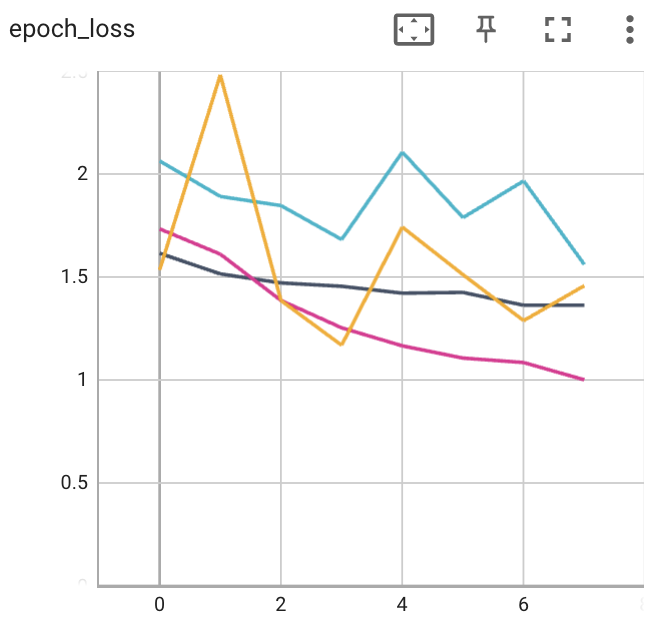
\includegraphics[width=\textwidth]{images/distilbert_loss.png}
    \end{minipage}
    \begin{minipage}[c]{0.4\textwidth}
        \caption{MSE loss values over the training of 8 epochs, on the training and validation datasets.}\label{fig:p2t-loss}
        \begin{itemize}
            \item \textbf{training} (grey \csq[HTML]{425066} for the \texttt{fixed} model, rose \csq[HTML]{e52592} for the \texttt{refined1} model),
            \item \textbf{validation} (blue \csq[HTML]{12b5cb} for the \texttt{fixed} model, orange \csq[HTML]{f9ab00} for the \texttt{refined1} model).
        \end{itemize}
        The \texttt{bottom1} model is not included for brevity.
    \end{minipage}
\end{figure}

\begin{figure}
    \centering
    \begin{subfigure}[t]{0.3\textwidth}
        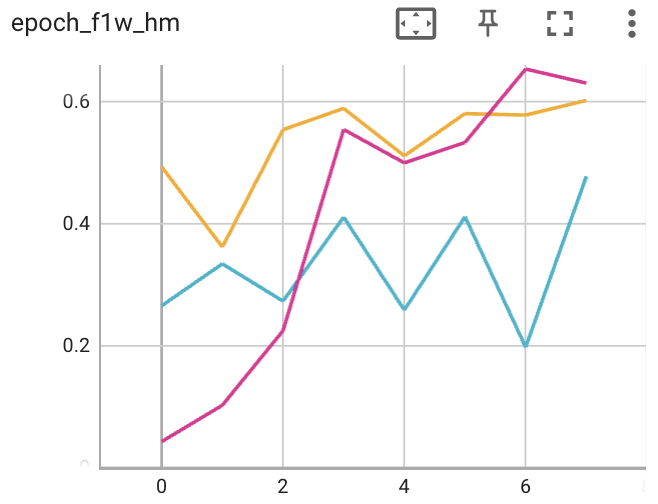
\includegraphics[width=\textwidth]{images/distilbert_val_f1w_hm.png}
        \caption{The harmonic mean of the Weighted-F1 scores of the two (positive, negative) sentiment variables.}
        \label{fig:p2t-val-metrics-hm}
    \end{subfigure}
    \hfill
    \begin{subfigure}[t]{0.3\textwidth}
        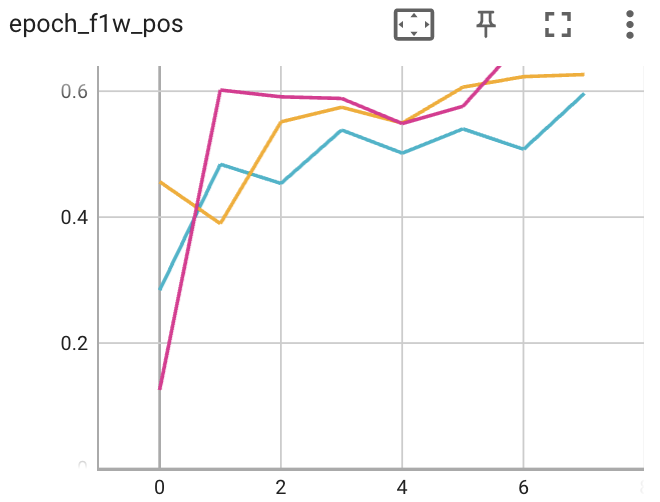
\includegraphics[width=\textwidth]{images/distilbert_val_f1w_pos.png}
        \caption{Weighted-F1 score of the positive sentiment variable.}
        \label{fig:p2t-val-metrics-pos}
    \end{subfigure}
    \hfill
    \begin{subfigure}[t]{0.3\textwidth}
        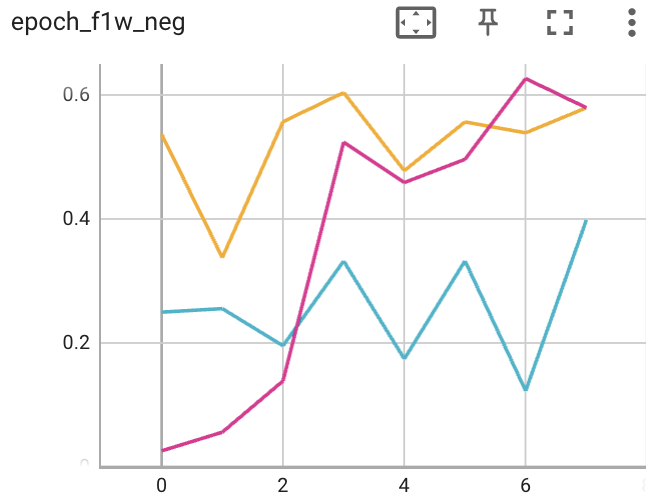
\includegraphics[width=\textwidth]{images/distilbert_val_f1w_neg.png}
        \caption{Weighted-F1 score of the negative sentiment variable.}
        \label{fig:p2t-val-metrics-neg}
    \end{subfigure}
    \caption{Three reported metrics for the positive (\cref{fig:p2t-val-metrics-pos}) and negative (\cref{fig:p2t-val-metrics-neg}) sentiment variables evaluated on the validation dataset, and their harmonic mean (\cref{fig:p2t-val-metrics-hm}, the main metric), after each of 8 training epochs.\\
    Blue \csq[HTML]{12b5cb} corresponds to the \texttt{fixed} model, orange \csq[HTML]{f9ab00} corresponds to the \texttt{refined1} model, and rose \csq[HTML]{e52592} corresponds to the \texttt{bottom1} model.}
    \label{fig:p2t-val-metrics}
\end{figure}

Suggested approaches to improve the performance if computational resources were not a bottleneck:
\begin{itemize}
    \item Train on a larger dataset. As described at the beginning of the section Transformers, we only consider 15\% of the provided dataset.
    \item Train for more epochs. As clearly seen from \cref{fig:p2t-val-metrics-hm} (harmonic weighted F1 grows) and \cref{fig:p2t-loss} (loss decreases), continuing the training for longer has a high predisposition for leading to better performance.
    \item Use a larger transformer model or allow fine-tuning of more layers of the selected model. Here, we opted for DistilBERT, which is a smaller, distilled version of BERT, but options with more layers (requiring more computing resources) have the potential to perform better. However, this approach would mostly make sense if the training reaches the bottleneck given by the complexity of the model.
\end{itemize}

\setcounter{section}{5}
\section{Embedding analysis}

In this question, we investigate what effect fine-tuning of the last layer of the pre-trained DistilBERT transformer model has on tweet embeddings. Therefore, we study the embeddings of tweets produced by two models, \texttt{fixed} (with all pre-trained layers fixed), and \texttt{refined1}, with the last pre-trained layer fine-tuned. First, we explain and clarify a few concepts used in this section.

\textbf{Tweet embeddings model.} Given a trained transformer model, we modify it such that it returns the embedding of the first token (\texttt{[CLS]}) of a given tweet. The transformer-based language models are trained such that the embedding of the \texttt{[CLS]} token (i.e. the first token after tokenisation) has information about the sentiment of the whole input sequence, that is why we choose to visualise the embedding of this token. Given a tweet, evaluating the model on the pre-processed and tokenized version of the tweet results in a 768-dimensional embedding of the tweet.

\textbf{Selected tweets: $\bm{1000 + 10}$.} We randomly sampled 1000 tweets from the test set (disjoint from the training set) to use for dimensionality reduction; not more due to computational constraints. For some visualisations in this section, we manually selected an additional set of ten tweets (also distinct from the 1000), which we manually verified are related to Covid-19. The embedding of those ten tweets can be visualised and annotated with the text. These ten tweets' whole (unprocessed and not tokenized) text is shown in \cref{tab:p2t-ten_tweets}.

\begin{table}[]
    \centering
    \setlength{\parindent}{-1em}
    \begin{tabular}{|r|p{16cm}|}
    \hline
1 & \negindent @TheMomKind This has happened to a few families...scary stuff... \\
2 & \negindent Joe Biden presents symptoms that ought to concern everyone. @DrBenChavis @NCPoliticalSpin @ChathCoLineNews @afaduln2 @mobygrapefan @Flwrgirl66x @Laura78703 @MaRobbie @shannondjackson @TulsiGabbard @ChuckRocha @TheBernReport @davidsirota @daviddoel @KyleKulinski @cenkuygur \\
3 & \negindent Coronavirus: Scientists say anti-parasite drug could kill virus https://t.co/BkRLwU12IR \\
4 & \negindent In these trying times when so many are testing positive for coronavirus we should have tremendous gratitude that Hillary Clinton still tests negative for president of the United States. \\
5 & \negindent Study out of New York may change everything we thought we knew about fevers and coronavirus   https://t.co/70yUs5HGNa \\
6 & \negindent Manchester City are approaching the situation with a \textquotedblleft{}clear, calm head\textquotedblright{}, according to senior sources, and have been laying the ground work for months in the event of a ban from UEFA. A robust legal challenge is expected to be lodged on appeal with CAS.  [@TeleFootball] \\
7 & \negindent I'm a little disappointed but shit happens \\
8 & \negindent I have been struggling to breathe with this Coronavirus. But I have been listening non stop to this worship song Unstoppable God by Sanctus Real. It has lifted my soul as Coronavirus attacked my lungs. Where does my help come, my help comes from the Lord. \#conronavirus \#COVID19 https://t.co/OEJrZvTv0J \\
9 & \negindent 44 migrants on one US deportation flight tested positive for coronavirus https://t.co/YqZDhacOWE \\
10 & \negindent I can't wait for that day when this pandemic is over.   Hoping for better days!\\
\hline
    \end{tabular}
    \caption{The full unprocessed text of ten selected tweets for visualisation purposes.}
    \label{tab:p2t-ten_tweets}
\end{table}

\textbf{Dimensionality reduction functions: PCA, UMAP.} When visualizing the ten selected tweets (\cref{tab:p2t-ten_tweets}), we need to use a dimensionality reduction function trained on a bigger sample set since 10 tweets alone would not be enough to capture the relationships of tweets in the whole test dataset. Therefore, we train the dimensionality reduction functions on the set of 1000 tweets. Further, we argue that the training of dimensionality reduction should be independent from the ten tweets that we later visualize, to avoid bias e.g. when setting the hyperparameters of the dimensionality reduction function. Thus, we opt for the methods PCA and UMAP \cite{umap}, which give us a function that we can apply to new data (as opposed to t-SNE \cite{tsne}, which cannot be applied to new data).

\Cref{fig:transformers_embeddings_diagram} shows the procedure to obtain visualisations of the two sets of selected tweets.

\begin{figure}
    \centering
    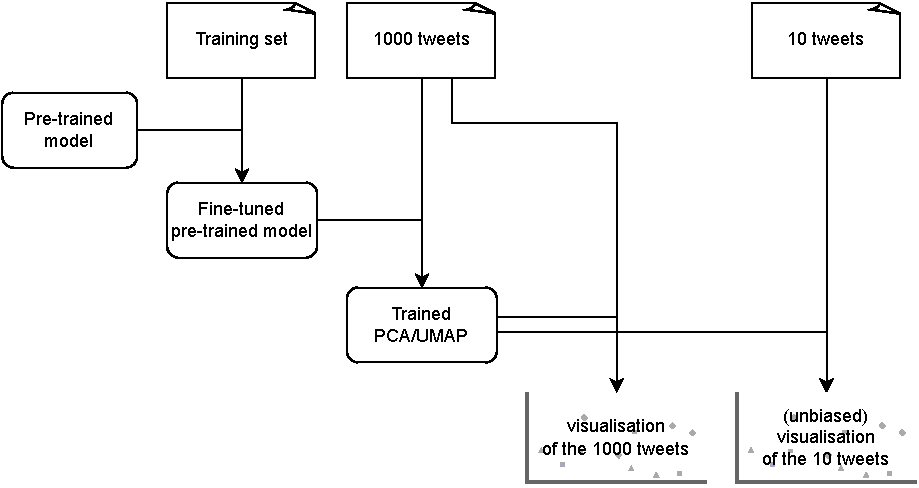
\includegraphics[width=11cm]{images/transformers_embeddings_diagram.pdf}
    \caption{Diagram showing how plots visualising tweet embeddings are obtained from three splits of the tweet dataset.}
    \label{fig:transformers_embeddings_diagram}
\end{figure}

\textbf{Positive sentiment}. In this section, we show plots where samples are colored by the positive sentiment variable. However, similar results and conclusions can be derived from plotting the negative sentiment variable; we don't include the plots for brevity.

As the first try, we tried to compare the embeddings of the 10 selected tweets, output by the two models \texttt{fixed} and \texttt{refined1}. This is visualized in \cref{fig:p2t-2models-embedding}. However, from inspecting the plots, we conclude that the fine-tuning of the model changes the meanings of the embedding dimensions enough such that combining tweet embeddings produced by the two models in the same embedding space doesn't convey useful information. In other words, the embedding space of the \texttt{refined1} model seems to have a different representation than the embedding space of the \texttt{fixed} model.

\begin{figure}
    \centering
    \begin{subfigure}[t]{\textwidth}
        \hspace*{1.5cm}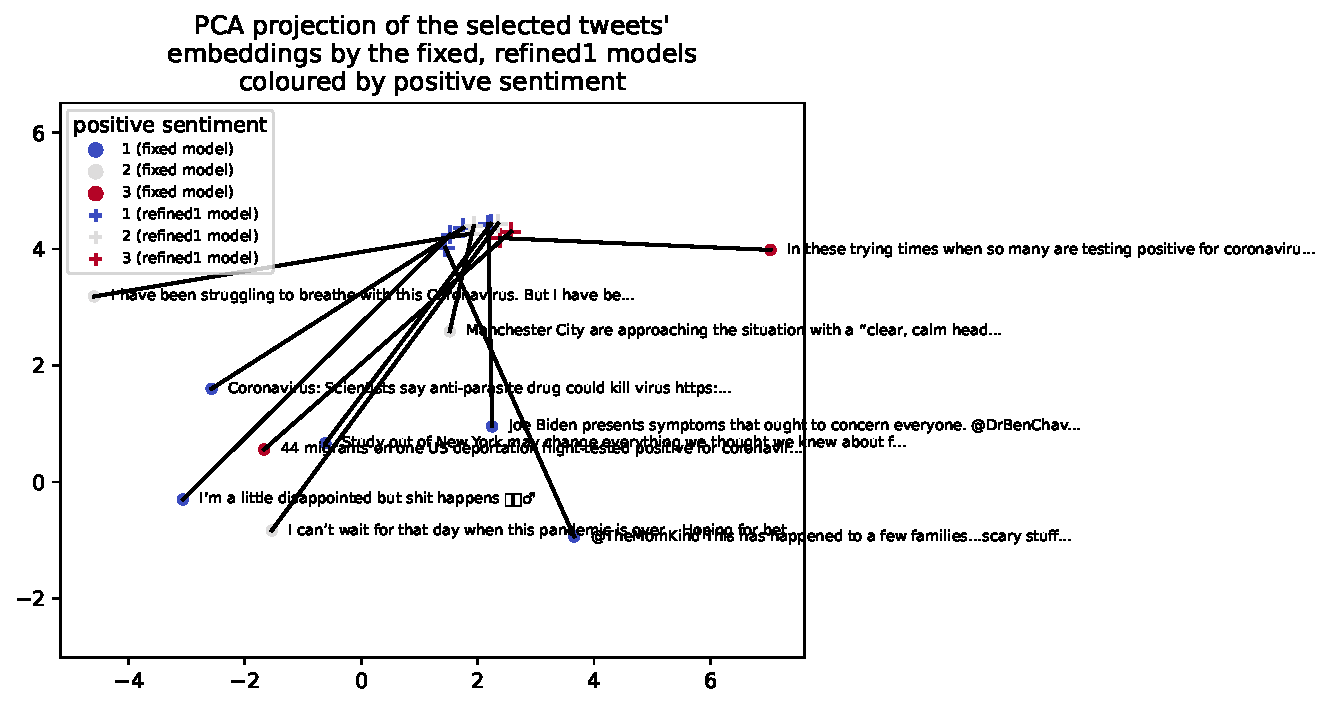
\includegraphics[height=9cm]{images/transformer_embedding2models_pca_positive.pdf}
        \caption{}\label{fig:p2t-2models-embedding-pca}
    \end{subfigure}
    \begin{subfigure}[t]{\textwidth}
        \hspace*{1.5cm}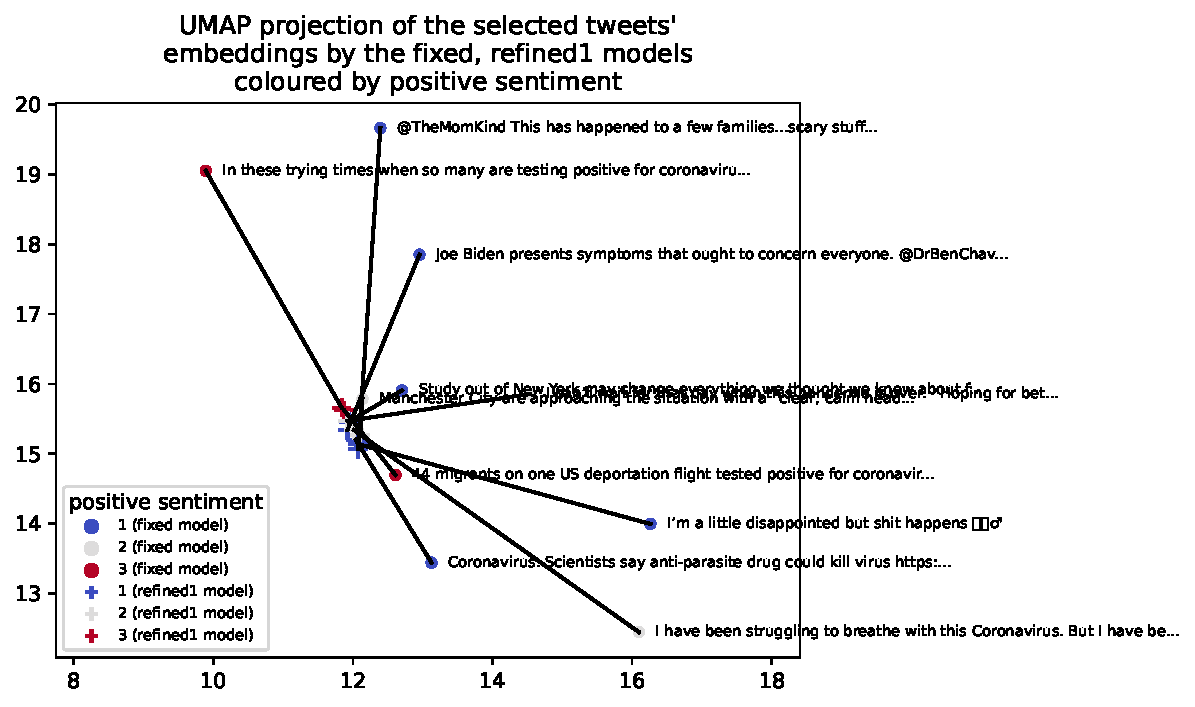
\includegraphics[height=9cm]{images/transformer_embedding2models_umap_positive.pdf}
        \caption{}\label{fig:p2t-2models-embedding-umap}
    \end{subfigure}
    \caption{Visualisation of the embeddings of the 10 selected tweets, output by the two models \texttt{fixed}, \texttt{refined1}. The dimensions are reduced to 2D using the same dimensionality reduction function (\cref{fig:p2t-2models-embedding-pca} PCA, \cref{fig:p2t-2models-embedding-umap} UMAP), trained on the 1000 embedding-tweets set output by the \texttt{fixed} model.}
    \label{fig:p2t-2models-embedding}
\end{figure}

On our second try, we visualised the embeddings separately for the two models. The result is shown in \cref{fig:p2t-embedding-fixed} (for the \texttt{fixed} model) and \cref{fig:p2t-embedding-refined1} (for the \texttt{refined1} model).
Finally, we also visualised all 1000 embedding vectors that were used to train the PCA and UMAP. Results are shown in \cref{fig:p2t-embeddings-many}.

The parameters set for UMAP in all visualisations in this section are \texttt{n\_neighbors=30}, \texttt{min\_dist=0.2}.

\begin{figure}
    \centering
    \begin{subfigure}[t]{\textwidth}
        \hspace*{1.5cm}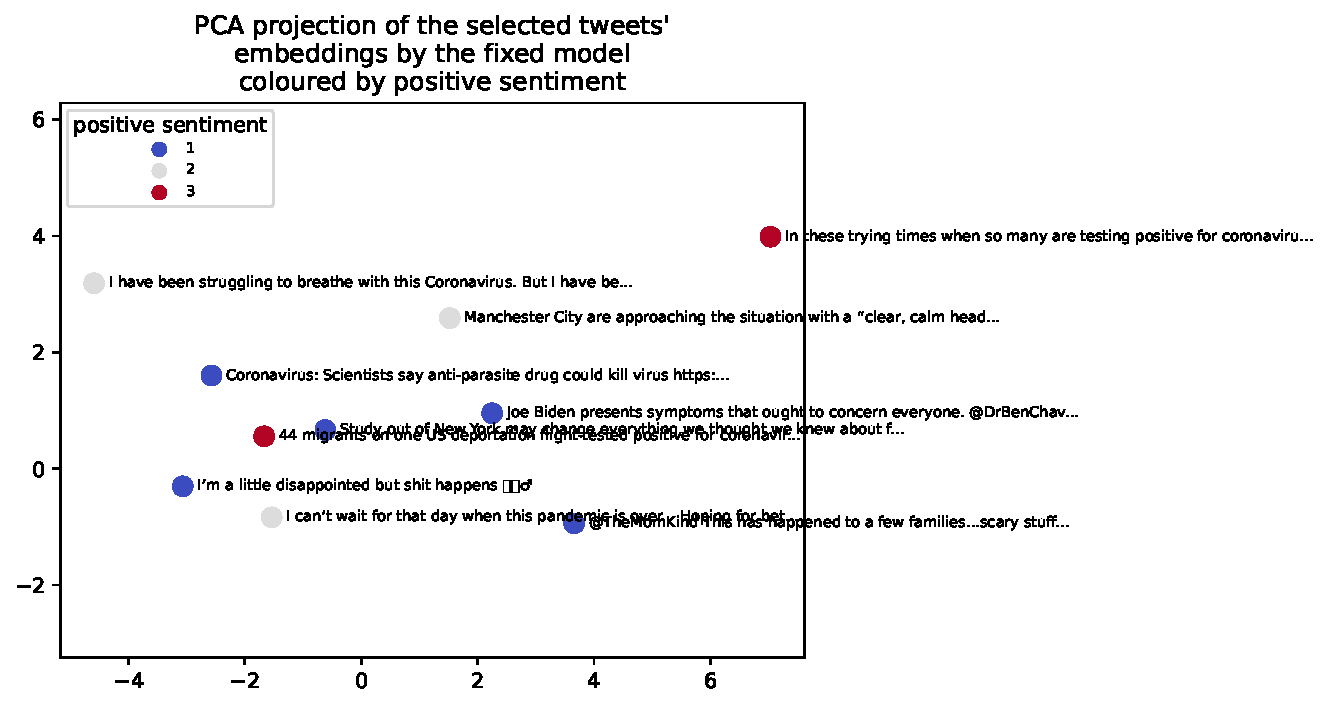
\includegraphics[height=9cm]{images/transformer_embedding_fixed_pca_positive.pdf}
        \caption{}\label{fig:p2t-embedding-fixed-pca}
    \end{subfigure}
    \begin{subfigure}[t]{\textwidth}
        \hspace*{1.5cm}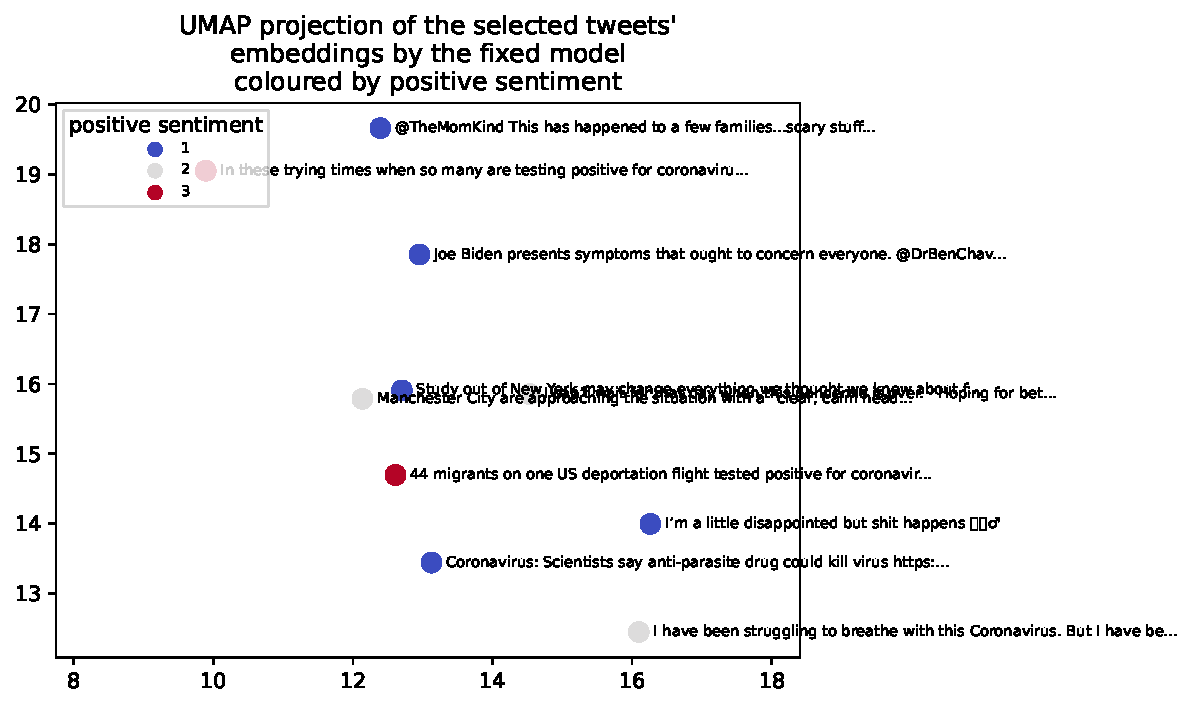
\includegraphics[height=9cm]{images/transformer_embedding_fixed_umap_positive.pdf}
        \caption{}\label{fig:p2t-embedding-fixed-umap}
    \end{subfigure}
    \caption{Visualisation of the embeddings of the 10 selected tweets, output by the \texttt{fixed} model, using \cref{fig:p2t-embedding-fixed-pca} PCA and \cref{fig:p2t-embedding-fixed-umap} UMAP dimensionality reduction functions trained on the 1000 embedding-tweets set output by the \texttt{fixed} model.}
    \label{fig:p2t-embedding-fixed}
\end{figure}
\begin{figure}
    \centering
    \begin{subfigure}[t]{\textwidth}
        \hspace*{1.5cm}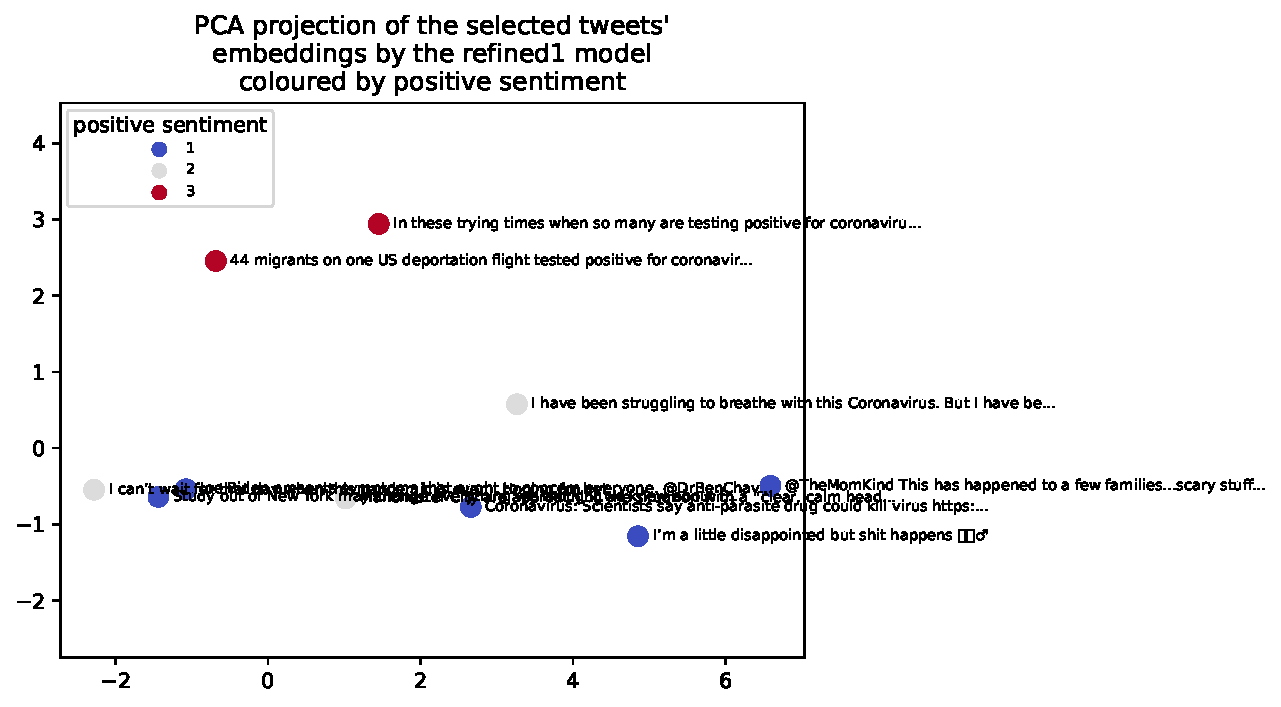
\includegraphics[height=9cm]{images/transformer_embedding_refined1_pca_positive.pdf}
        \caption{}\label{fig:p2t-embedding-refined1-pca}
    \end{subfigure}
    \begin{subfigure}[t]{\textwidth}
        \hspace*{1.5cm}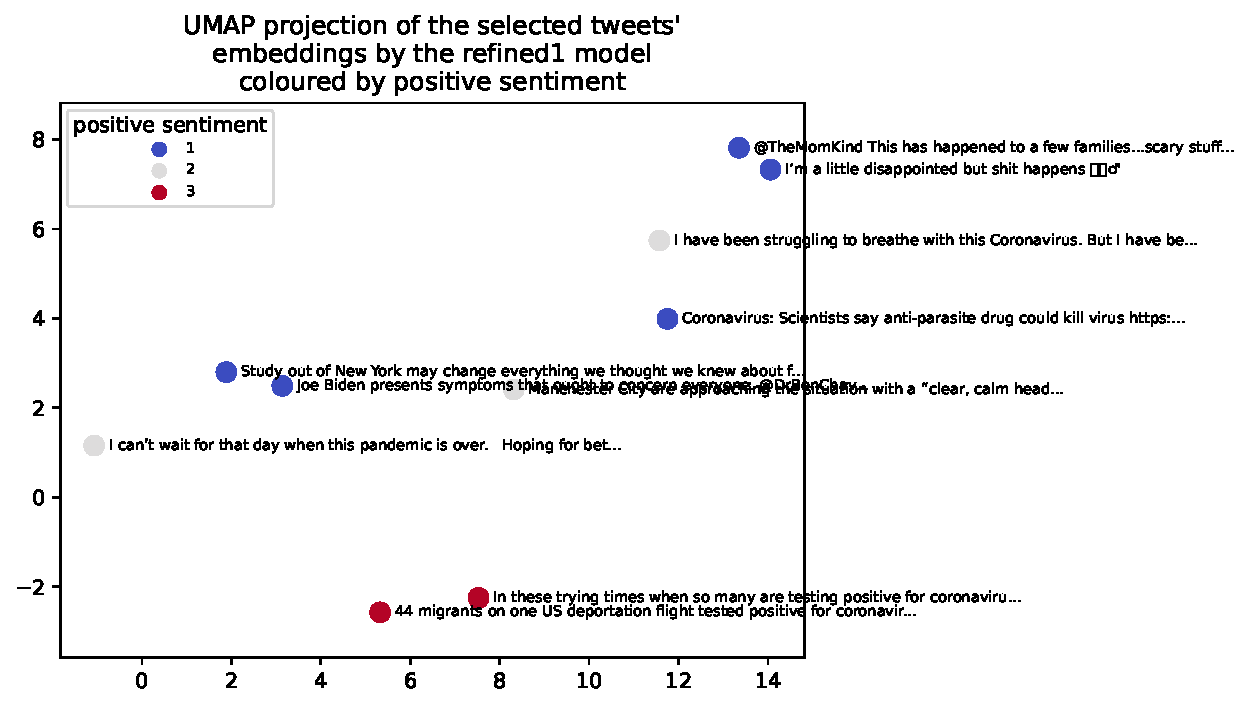
\includegraphics[height=9cm]{images/transformer_embedding_refined1_umap_positive.pdf}
        \caption{}\label{fig:p2t-embedding-refined1-umap}
    \end{subfigure}
    \caption{Visualisation of the embeddings of the 10 selected tweets, output by the \texttt{refined1} model, using \cref{fig:p2t-embedding-refined1-pca} PCA and \cref{fig:p2t-embedding-refined1-umap} UMAP dimensionality reduction functions trained on the 1000 embedding-tweets set output by the \texttt{refined1} model.}
    \label{fig:p2t-embedding-refined1}
\end{figure}

\begin{figure}
    \centering
    \begin{subfigure}{0.49\textwidth}
        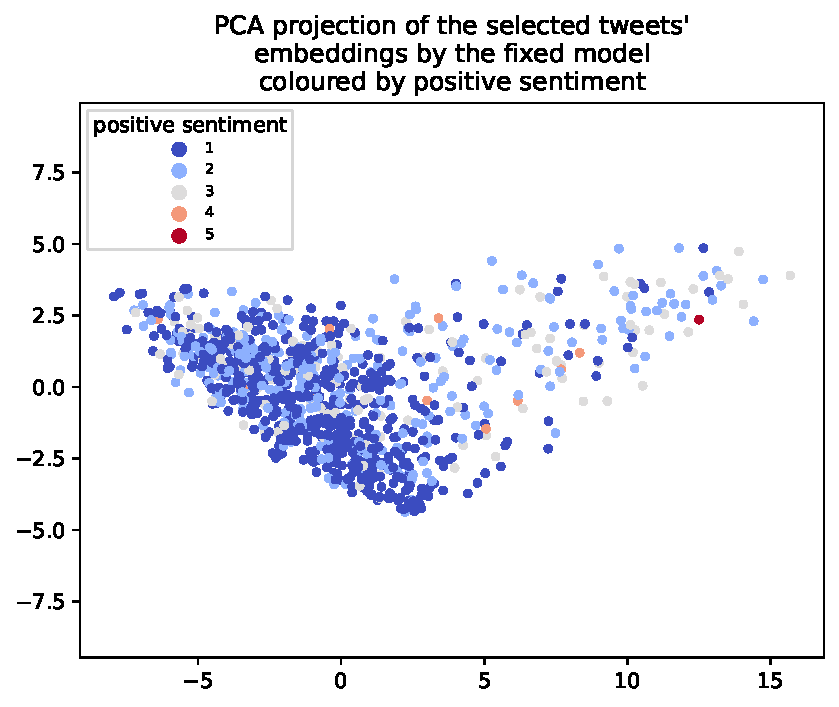
\includegraphics[width=\textwidth]{images/transformer_embedding_many_fixed_pca_positive.pdf}
        \caption{}\label{fig:p2t-embeddings-many-fixed-pca}
    \end{subfigure}
    \hfill
    \begin{subfigure}{0.49\textwidth}
        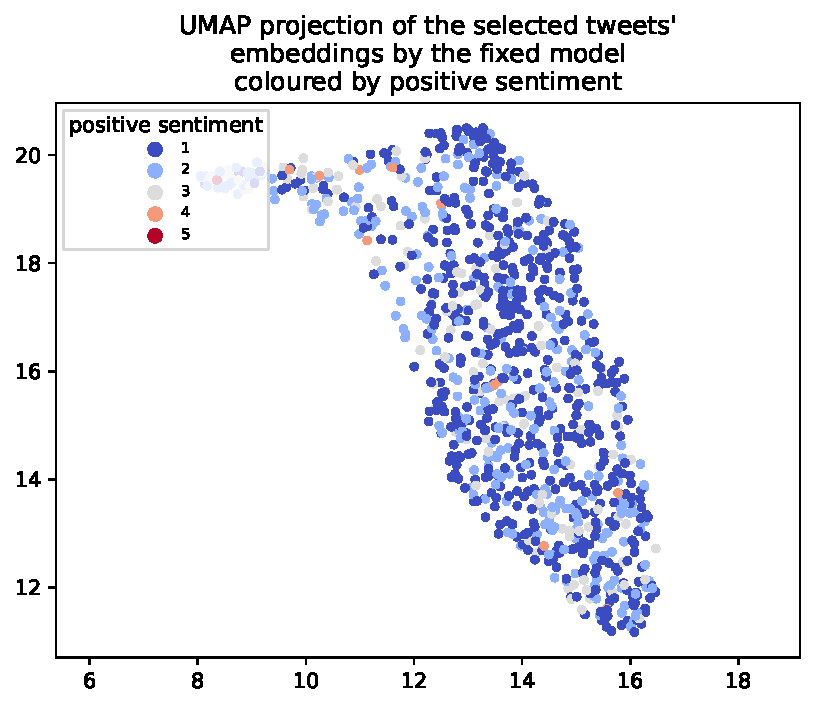
\includegraphics[width=\textwidth]{images/transformer_embedding_many_fixed_umap_positive.pdf}
        \caption{}\label{fig:p2t-embeddings-many-fixed-umap}
    \end{subfigure}
    \begin{subfigure}{0.49\textwidth}
        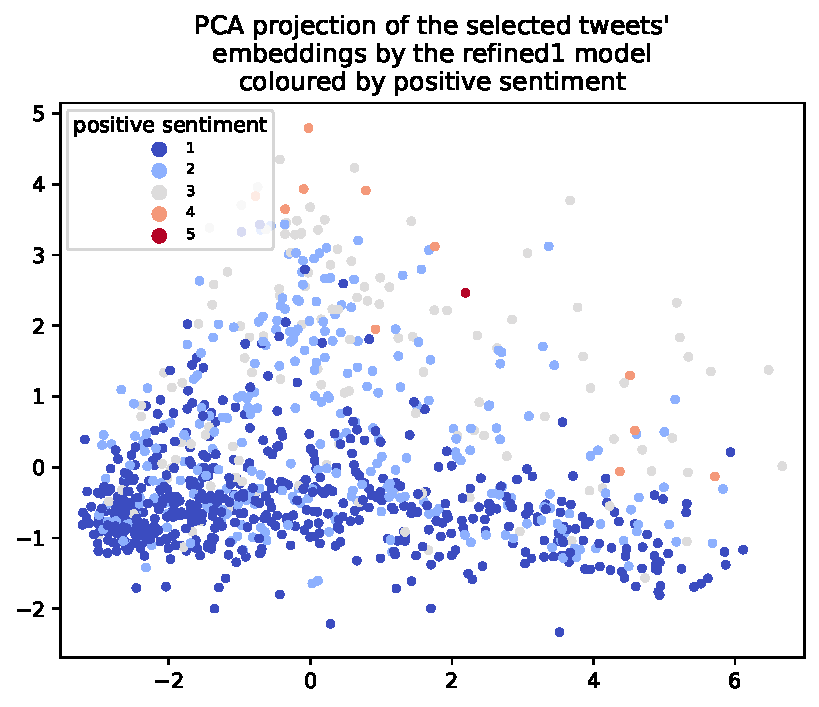
\includegraphics[width=\textwidth]{images/transformer_embedding_many_refined1_pca_positive.pdf}
        \caption{}\label{fig:p2t-embeddings-many-refined1-pca}
    \end{subfigure}
    \hfill
    \begin{subfigure}{0.49\textwidth}
        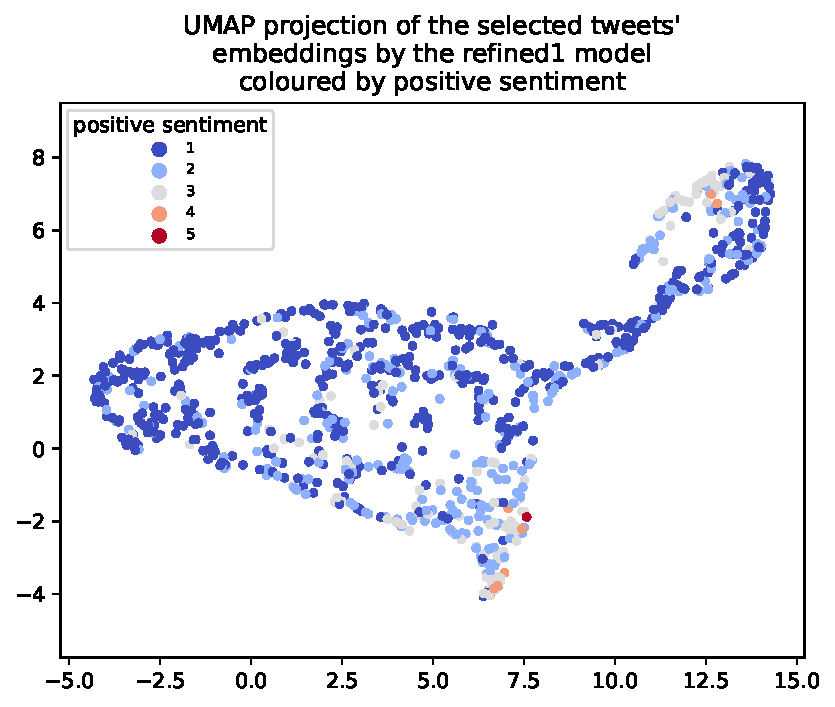
\includegraphics[width=\textwidth]{images/transformer_embedding_many_refined1_umap_positive.pdf}
        \caption{}\label{fig:p2t-embeddings-many-refined1-umap}
    \end{subfigure}
    \caption{Visualisation of PCA and UMAP values of the 1000 embeddings that were used to train the dimensionality reduction functions. Results are shown for models \texttt{fixed} (\cref{fig:p2t-embeddings-many-fixed-pca} PCA, \cref{fig:p2t-embeddings-many-fixed-umap} UMAP), \texttt{refined} (\cref{fig:p2t-embeddings-many-refined1-pca} PCA, \cref{fig:p2t-embeddings-many-refined1-umap} UMAP).}
    \label{fig:p2t-embeddings-many}
\end{figure}

\textbf{Conclusions.}
In the scatter plots, we can observe the following: None of the PCA and UMAP plots of the embeddings from the \texttt{fixed} model (i.e. \cref{fig:p2t-embedding-fixed}, \cref{fig:p2t-embeddings-many-fixed-pca}, \cref{fig:p2t-embeddings-many-fixed-umap}) show any clustering related to the positive sentiment, in that tweets of all positive-sentiment values, are distributed relatively uniformly across the embedding space.
This may be a natural consequence of the fact that these embeddings are produced by a pre-trained model.
During training for our task (regression of two sentiment values), we only trained the weights of two layers built on top of the tweet embedding. Thus, no weights that affect the embedding were changed during this training, and so the embedding of tweets is exactly as would be output by the original pre-trained model.
One might still expect the embedding to convey information relevant to sentiment prediction since the used model \texttt{"distilbert-base-uncased-finetuned-sst-2-english"} is pre-trained on the Stanford Sentiment Treebank \cite{socherRecursiveDeepModels2013} corpora. However, apparently, the original problem and the problem in this project are different enough.

However, in scatter plots of embeddings from the \texttt{refined1} model (\cref{fig:p2t-embedding-refined1}, \cref{fig:p2t-embeddings-many-refined1-pca}, \cref{fig:p2t-embeddings-many-refined1-umap}), we see the separation of tweets based on their positive sentiment value, while the only connection between those scatter plots and the positive sentiment variable is that the last pre-trained layer of the \texttt{refined1} model was fine-tuned to predict the positive and negative sentiment variables.
As a specific example, the $y$-axis of the PCA plot in \cref{fig:p2t-embeddings-many-refined1-pca} is highly correlated with the positive sentiment variable: tweets labelled with high positive sentiment are mostly present at higher $y$ values in the plot.
Further, in the UMAP in \cref{fig:p2t-embeddings-many-refined1-umap}, tweets with higher positive sentiment values are nicely separated from the low-positive-sentiment tweets, and so even a clustering algorithm on the 2D UMAP would likely lead to better-than-random performance.
As demonstrated, it suffices to fine-tune the last layer (the ultimate pre-embedding layer) to make the embeddings specialised and convey information about the positive sentiment variable.
We conclude that fine-tuning the model does result in the embeddings being more specialized for the given task.

Compared to visualising word embeddings in Part 2, Q6, we see that the separation of positive and negative tweets using transformer-based models is visually stronger than the separation of positive and negative words as shown in Part 2, Q6, where the performance of a simple clustering algorithm on the 2D embedding would likely be poor.
